
%% bare_jrnl_compsoc.tex
%% V1.4a
%% 2014/09/17
%% by Michael Shell
%% See:
%% http://www.michaelshell.org/
%% for current contact information.
%%
%% This is a skeleton file demonstrating the use of IEEEtran.cls
%% (requires IEEEtran.cls version 1.8a or later) with an IEEE
%% Computer Society journal paper.
%%
%% Support sites:
%% http://www.michaelshell.org/tex/ieeetran/
%% http://www.ctan.org/tex-archive/macros/latex/contrib/IEEEtran/
%% and
%% http://www.ieee.org/

%%*************************************************************************
%% Legal Notice:
%% This code is offered as-is without any warranty either expressed or
%% implied; without even the implied warranty of MERCHANTABILITY or
%% FITNESS FOR A PARTICULAR PURPOSE! 
%% User assumes all risk.
%% In no event shall IEEE or any contributor to this code be liable for
%% any damages or losses, including, but not limited to, incidental,
%% consequential, or any other damages, resulting from the use or misuse
%% of any information contained here.
%%
%% All comments are the opinions of their respective authors and are not
%% necessarily endorsed by the IEEE.
%%
%% This work is distributed under the LaTeX Project Public License (LPPL)
%% ( http://www.latex-project.org/ ) version 1.3, and may be freely used,
%% distributed and modified. A copy of the LPPL, version 1.3, is included
%% in the base LaTeX documentation of all distributions of LaTeX released
%% 2003/12/01 or later.
%% Retain all contribution notices and credits.
%% ** Modified files should be clearly indicated as such, including  **
%% ** renaming them and changing author support contact information. **
%%
%% File list of work: IEEEtran.cls, IEEEtran_HOWTO.pdf, bare_adv.tex,
%%                    bare_conf.tex, bare_jrnl.tex, bare_conf_compsoc.tex,
%%                    bare_jrnl_compsoc.tex, bare_jrnl_transmag.tex
%%*************************************************************************


% *** Authors should verify (and, if needed, correct) their LaTeX system  ***
% *** with the testflow diagnostic prior to trusting their LaTeX platform ***
% *** with production work. IEEE's font choices and paper sizes can       ***
% *** trigger bugs that do not appear when using other class files.       ***                          ***
% The testflow support page is at:
% http://www.michaelshell.org/tex/testflow/


\documentclass[10pt,journal,compsoc]{IEEEtran}
%
% If IEEEtran.cls has not been installed into the LaTeX system files,
% manually specify the path to it like:
% \documentclass[10pt,journal,compsoc]{../sty/IEEEtran}





% Some very useful LaTeX packages include:
% (uncomment the ones you want to load)


% *** MISC UTILITY PACKAGES ***
%
%\usepackage{ifpdf}
% Heiko Oberdiek's ifpdf.sty is very useful if you need conditional
% compilation based on whether the output is pdf or dvi.
% usage:
% \ifpdf
%   % pdf code
% \else
%   % dvi code
% \fi
% The latest version of ifpdf.sty can be obtained from:
% http://www.ctan.org/tex-archive/macros/latex/contrib/oberdiek/
% Also, note that IEEEtran.cls V1.7 and later provides a builtin
% \ifCLASSINFOpdf conditional that works the same way.
% When switching from latex to pdflatex and vice-versa, the compiler may
% have to be run twice to clear warning/error messages.






% *** CITATION PACKAGES ***
%
\ifCLASSOPTIONcompsoc
  % IEEE Computer Society needs nocompress option
  % requires cite.sty v4.0 or later (November 2003)
  \usepackage[nocompress]{cite}
\else
  % normal IEEE
  \usepackage{cite}
\fi
% cite.sty was written by Donald Arseneau
% V1.6 and later of IEEEtran pre-defines the format of the cite.sty package
% \cite{} output to follow that of IEEE. Loading the cite package will
% result in citation numbers being automatically sorted and properly
% "compressed/ranged". e.g., [1], [9], [2], [7], [5], [6] without using
% cite.sty will become [1], [2], [5]--[7], [9] using cite.sty. cite.sty's
% \cite will automatically add leading space, if needed. Use cite.sty's
% noadjust option (cite.sty V3.8 and later) if you want to turn this off
% such as if a citation ever needs to be enclosed in parenthesis.
% cite.sty is already installed on most LaTeX systems. Be sure and use
% version 5.0 (2009-03-20) and later if using hyperref.sty.
% The latest version can be obtained at:
% http://www.ctan.org/tex-archive/macros/latex/contrib/cite/
% The documentation is contained in the cite.sty file itself.
%
% Note that some packages require special options to format as the Computer
% Society requires. In particular, Computer Society  papers do not use
% compressed citation ranges as is done in typical IEEE papers
% (e.g., [1]-[4]). Instead, they list every citation separately in order
% (e.g., [1], [2], [3], [4]). To get the latter we need to load the cite
% package with the nocompress option which is supported by cite.sty v4.0
% and later. Note also the use of a CLASSOPTION conditional provided by
% IEEEtran.cls V1.7 and later.





% *** GRAPHICS RELATED PACKAGES ***
%
\ifCLASSINFOpdf
  % \usepackage[pdftex]{graphicx}
  % declare the path(s) where your graphic files are
  % \graphicspath{{../pdf/}{../jpeg/}}
  % and their extensions so you won't have to specify these with
  % every instance of \includegraphics
  % \DeclareGraphicsExtensions{.pdf,.jpeg,.png}
\else
  % or other class option (dvipsone, dvipdf, if not using dvips). graphicx
  % will default to the driver specified in the system graphics.cfg if no
  % driver is specified.
  % \usepackage[dvips]{graphicx}
  % declare the path(s) where your graphic files are
  % \graphicspath{{../eps/}}
  % and their extensions so you won't have to specify these with
  % every instance of \includegraphics
  % \DeclareGraphicsExtensions{.eps}
\fi
% graphicx was written by David Carlisle and Sebastian Rahtz. It is
% required if you want graphics, photos, etc. graphicx.sty is already
% installed on most LaTeX systems. The latest version and documentation
% can be obtained at: 
% http://www.ctan.org/tex-archive/macros/latex/required/graphics/
% Another good source of documentation is "Using Imported Graphics in
% LaTeX2e" by Keith Reckdahl which can be found at:
% http://www.ctan.org/tex-archive/info/epslatex/
%
% latex, and pdflatex in dvi mode, support graphics in encapsulated
% postscript (.eps) format. pdflatex in pdf mode supports graphics
% in .pdf, .jpeg, .png and .mps (metapost) formats. Users should ensure
% that all non-photo figures use a vector format (.eps, .pdf, .mps) and
% not a bitmapped formats (.jpeg, .png). IEEE frowns on bitmapped formats
% which can result in "jaggedy"/blurry rendering of lines and letters as
% well as large increases in file sizes.
%
% You can find documentation about the pdfTeX application at:
% http://www.tug.org/applications/pdftex






% *** MATH PACKAGES ***
%
%\usepackage[cmex10]{amsmath}
% A popular package from the American Mathematical Society that provides
% many useful and powerful commands for dealing with mathematics. If using
% it, be sure to load this package with the cmex10 option to ensure that
% only type 1 fonts will utilized at all point sizes. Without this option,
% it is possible that some math symbols, particularly those within
% footnotes, will be rendered in bitmap form which will result in a
% document that can not be IEEE Xplore compliant!
%
% Also, note that the amsmath package sets \interdisplaylinepenalty to 10000
% thus preventing page breaks from occurring within multiline equations. Use:
%\interdisplaylinepenalty=2500
% after loading amsmath to restore such page breaks as IEEEtran.cls normally
% does. amsmath.sty is already installed on most LaTeX systems. The latest
% version and documentation can be obtained at:
% http://www.ctan.org/tex-archive/macros/latex/required/amslatex/math/





% *** SPECIALIZED LIST PACKAGES ***
%
%\usepackage{algorithmic}
% algorithmic.sty was written by Peter Williams and Rogerio Brito.
% This package provides an algorithmic environment fo describing algorithms.
% You can use the algorithmic environment in-text or within a figure
% environment to provide for a floating algorithm. Do NOT use the algorithm
% floating environment provided by algorithm.sty (by the same authors) or
% algorithm2e.sty (by Christophe Fiorio) as IEEE does not use dedicated
% algorithm float types and packages that provide these will not provide
% correct IEEE style captions. The latest version and documentation of
% algorithmic.sty can be obtained at:
% http://www.ctan.org/tex-archive/macros/latex/contrib/algorithms/
% There is also a support site at:
% http://algorithms.berlios.de/index.html
% Also of interest may be the (relatively newer and more customizable)
% algorithmicx.sty package by Szasz Janos:
% http://www.ctan.org/tex-archive/macros/latex/contrib/algorithmicx/




% *** ALIGNMENT PACKAGES ***
%
%\usepackage{array}
% Frank Mittelbach's and David Carlisle's array.sty patches and improves
% the standard LaTeX2e array and tabular environments to provide better
% appearance and additional user controls. As the default LaTeX2e table
% generation code is lacking to the point of almost being broken with
% respect to the quality of the end results, all users are strongly
% advised to use an enhanced (at the very least that provided by array.sty)
% set of table tools. array.sty is already installed on most systems. The
% latest version and documentation can be obtained at:
% http://www.ctan.org/tex-archive/macros/latex/required/tools/


% IEEEtran contains the IEEEeqnarray family of commands that can be used to
% generate multiline equations as well as matrices, tables, etc., of high
% quality.




% *** SUBFIGURE PACKAGES ***
%\ifCLASSOPTIONcompsoc
%  \usepackage[caption=false,font=footnotesize,labelfont=sf,textfont=sf]{subfig}
%\else
%  \usepackage[caption=false,font=footnotesize]{subfig}
%\fi
% subfig.sty, written by Steven Douglas Cochran, is the modern replacement
% for subfigure.sty, the latter of which is no longer maintained and is
% incompatible with some LaTeX packages including fixltx2e. However,
% subfig.sty requires and automatically loads Axel Sommerfeldt's caption.sty
% which will override IEEEtran.cls' handling of captions and this will result
% in non-IEEE style figure/table captions. To prevent this problem, be sure
% and invoke subfig.sty's "caption=false" package option (available since
% subfig.sty version 1.3, 2005/06/28) as this is will preserve IEEEtran.cls
% handling of captions.
% Note that the Computer Society format requires a sans serif font rather
% than the serif font used in traditional IEEE formatting and thus the need
% to invoke different subfig.sty package options depending on whether
% compsoc mode has been enabled.
%
% The latest version and documentation of subfig.sty can be obtained at:
% http://www.ctan.org/tex-archive/macros/latex/contrib/subfig/




% *** FLOAT PACKAGES ***
%
%\usepackage{fixltx2e}
% fixltx2e, the successor to the earlier fix2col.sty, was written by
% Frank Mittelbach and David Carlisle. This package corrects a few problems
% in the LaTeX2e kernel, the most notable of which is that in current
% LaTeX2e releases, the ordering of single and double column floats is not
% guaranteed to be preserved. Thus, an unpatched LaTeX2e can allow a
% single column figure to be placed prior to an earlier double column
% figure. The latest version and documentation can be found at:
% http://www.ctan.org/tex-archive/macros/latex/base/


%\usepackage{stfloats}
% stfloats.sty was written by Sigitas Tolusis. This package gives LaTeX2e
% the ability to do double column floats at the bottom of the page as well
% as the top. (e.g., "\begin{figure*}[!b]" is not normally possible in
% LaTeX2e). It also provides a command:
%\fnbelowfloat
% to enable the placement of footnotes below bottom floats (the standard
% LaTeX2e kernel puts them above bottom floats). This is an invasive package
% which rewrites many portions of the LaTeX2e float routines. It may not work
% with other packages that modify the LaTeX2e float routines. The latest
% version and documentation can be obtained at:
% http://www.ctan.org/tex-archive/macros/latex/contrib/sttools/
% Do not use the stfloats baselinefloat ability as IEEE does not allow
% \baselineskip to stretch. Authors submitting work to the IEEE should note
% that IEEE rarely uses double column equations and that authors should try
% to avoid such use. Do not be tempted to use the cuted.sty or midfloat.sty
% packages (also by Sigitas Tolusis) as IEEE does not format its papers in
% such ways.
% Do not attempt to use stfloats with fixltx2e as they are incompatible.
% Instead, use Morten Hogholm'a dblfloatfix which combines the features
% of both fixltx2e and stfloats:
%
% \usepackage{dblfloatfix}
% The latest version can be found at:
% http://www.ctan.org/tex-archive/macros/latex/contrib/dblfloatfix/




%\ifCLASSOPTIONcaptionsoff
%  \usepackage[nomarkers]{endfloat}
% \let\MYoriglatexcaption\caption
% \renewcommand{\caption}[2][\relax]{\MYoriglatexcaption[#2]{#2}}
%\fi
% endfloat.sty was written by James Darrell McCauley, Jeff Goldberg and 
% Axel Sommerfeldt. This package may be useful when used in conjunction with 
% IEEEtran.cls'  captionsoff option. Some IEEE journals/societies require that
% submissions have lists of figures/tables at the end of the paper and that
% figures/tables without any captions are placed on a page by themselves at
% the end of the document. If needed, the draftcls IEEEtran class option or
% \CLASSINPUTbaselinestretch interface can be used to increase the line
% spacing as well. Be sure and use the nomarkers option of endfloat to
% prevent endfloat from "marking" where the figures would have been placed
% in the text. The two hack lines of code above are a slight modification of
% that suggested by in the endfloat docs (section 8.4.1) to ensure that
% the full captions always appear in the list of figures/tables - even if
% the user used the short optional argument of \caption[]{}.
% IEEE papers do not typically make use of \caption[]'s optional argument,
% so this should not be an issue. A similar trick can be used to disable
% captions of packages such as subfig.sty that lack options to turn off
% the subcaptions:
% For subfig.sty:
% \let\MYorigsubfloat\subfloat
% \renewcommand{\subfloat}[2][\relax]{\MYorigsubfloat[]{#2}}
% However, the above trick will not work if both optional arguments of
% the \subfloat command are used. Furthermore, there needs to be a
% description of each subfigure *somewhere* and endfloat does not add
% subfigure captions to its list of figures. Thus, the best approach is to
% avoid the use of subfigure captions (many IEEE journals avoid them anyway)
% and instead reference/explain all the subfigures within the main caption.
% The latest version of endfloat.sty and its documentation can obtained at:
% http://www.ctan.org/tex-archive/macros/latex/contrib/endfloat/
%
% The IEEEtran \ifCLASSOPTIONcaptionsoff conditional can also be used
% later in the document, say, to conditionally put the References on a 
% page by themselves.




% *** PDF, URL AND HYPERLINK PACKAGES ***
%
\usepackage{url}
% url.sty was written by Donald Arseneau. It provides better support for
% handling and breaking URLs. url.sty is already installed on most LaTeX
% systems. The latest version and documentation can be obtained at:
% http://www.ctan.org/tex-archive/macros/latex/contrib/url/
% Basically, \url{my_url_here}.

\usepackage[utf8]{inputenc}
\usepackage[T1]{fontenc}
\usepackage[spanish]{babel}
\usepackage{graphicx}
\graphicspath{ {images/} }



% *** Do not adjust lengths that control margins, column widths, etc. ***
% *** Do not use packages that alter fonts (such as pslatex).         ***
% There should be no need to do such things with IEEEtran.cls V1.6 and later.
% (Unless specifically asked to do so by the journal or conference you plan
% to submit to, of course. )


% correct bad hyphenation here
\hyphenation{op-tical net-works semi-conduc-tor}


\begin{document}
%
% paper title
% Titles are generally capitalized except for words such as a, an, and, as,
% at, but, by, for, in, nor, of, on, or, the, to and up, which are usually
% not capitalized unless they are the first or last word of the title.
% Linebreaks \\ can be used within to get better formatting as desired.
% Do not put math or special symbols in the title.
\title{Software Defined Networks}
%
%
% author names and IEEE memberships
% note positions of commas and nonbreaking spaces ( ~ ) LaTeX will not break
% a structure at a ~ so this keeps an author's name from being broken across
% two lines.
% use \thanks{} to gain access to the first footnote area
% a separate \thanks must be used for each paragraph as LaTeX2e's \thanks
% was not built to handle multiple paragraphs
%
%
%\IEEEcompsocitemizethanks is a special \thanks that produces the bulleted
% lists the Computer Society journals use for "first footnote" author
% affiliations. Use \IEEEcompsocthanksitem which works much like \item
% for each affiliation group. When not in compsoc mode,
% \IEEEcompsocitemizethanks becomes like \thanks and
% \IEEEcompsocthanksitem becomes a line break with idention. This
% facilitates dual compilation, although admittedly the differences in the
% desired content of \author between the different types of papers makes a
% one-size-fits-all approach a daunting prospect. For instance, compsoc 
% journal papers have the author affiliations above the "Manuscript
% received ..."  text while in non-compsoc journals this is reversed. Sigh.



% note the % following the last \IEEEmembership and also \thanks - 
% these prevent an unwanted space from occurring between the last author name
% and the end of the author line. i.e., if you had this:
% 
% \author{....lastname \thanks{...} \thanks{...} }
%                     ^------------^------------^----Do not want these spaces!
%
% a space would be appended to the last name and could cause every name on that
% line to be shifted left slightly. This is one of those "LaTeX things". For
% instance, "\textbf{A} \textbf{B}" will typeset as "A B" not "AB". To get
% "AB" then you have to do: "\textbf{A}\textbf{B}"
% \thanks is no different in this regard, so shield the last } of each \thanks
% that ends a line with a % and do not let a space in before the next \thanks.
% Spaces after \IEEEmembership other than the last one are OK (and needed) as
% you are supposed to have spaces between the names. For what it is worth,
% this is a minor point as most people would not even notice if the said evil
% space somehow managed to creep in.

\author{\IEEEauthorblockN{Priscilla~Piedra y Martín~Flores}\\
        \IEEEauthorblockA{
        Escuela de Ingeniería en Computación\\
        Instituto Tecnológico de Costa Rica. Cartago, Costa Rica
        }\\
        \small{\texttt{\{ppiedra90, mfloresg\}}\texttt{@gmail.com}}% <-this % stops a space
\thanks{Este documento fue realizado durante el curso Redes de Computadoras Avanzadas, impartido por el profesor Luis Carlos Loaiza Canet. Programa de Maestría en Computación, Instituto Tecnológico de Costa Rica. Segundo Semestre, 2017.}
}

% The paper headers
%\markboth{Journal of \LaTeX\ Class Files,~Vol.~13, No.~9, September~2014}%
%{Shell \MakeLowercase{\textit{et al.}}: Bare Demo of IEEEtran.cls for Computer Society Journals}

\markboth{Redes de Computadoras Avanzadas, Agosto 2017}%
{Shell \MakeLowercase{\textit{et al.}}: Bare Demo of IEEEtran.cls for Computer Society Journals}


% The only time the second header will appear is for the odd numbered pages
% after the title page when using the twoside option.
% 
% *** Note that you probably will NOT want to include the author's ***
% *** name in the headers of peer review papers.                   ***
% You can use \ifCLASSOPTIONpeerreview for conditional compilation here if
% you desire.



% The publisher's ID mark at the bottom of the page is less important with
% Computer Society journal papers as those publications place the marks
% outside of the main text columns and, therefore, unlike regular IEEE
% journals, the available text space is not reduced by their presence.
% If you want to put a publisher's ID mark on the page you can do it like
% this:
%\IEEEpubid{0000--0000/00\$00.00~\copyright~2014 IEEE}
% or like this to get the Computer Society new two part style.
%\IEEEpubid{\makebox[\columnwidth]{\hfill 0000--0000/00/\$00.00~\copyright~2014 IEEE}%
%\hspace{\columnsep}\makebox[\columnwidth]{Published by the IEEE Computer Society\hfill}}
% Remember, if you use this you must call \IEEEpubidadjcol in the second
% column for its text to clear the IEEEpubid mark (Computer Society jorunal
% papers don't need this extra clearance.)



% use for special paper notices
%\IEEEspecialpapernotice{(Invited Paper)}



% for Computer Society papers, we must declare the abstract and index terms
% PRIOR to the title within the \IEEEtitleabstractindextext IEEEtran
% command as these need to go into the title area created by \maketitle.
% As a general rule, do not put math, special symbols or citations
% in the abstract or keywords.
\IEEEtitleabstractindextext{%
\begin{abstract}
Aquí va el abstract
\end{abstract}

% Note that keywords are not normally used for peerreview papers.
%\begin{IEEEkeywords}
%Computer Society, IEEEtran, journal, \LaTeX, paper, template.
%\end{IEEEkeywords}
}


% make the title area
\maketitle


% To allow for easy dual compilation without having to reenter the
% abstract/keywords data, the \IEEEtitleabstractindextext text will
% not be used in maketitle, but will appear (i.e., to be "transported")
% here as \IEEEdisplaynontitleabstractindextext when the compsoc 
% or transmag modes are not selected <OR> if conference mode is selected 
% - because all conference papers position the abstract like regular
% papers do.
\IEEEdisplaynontitleabstractindextext
% \IEEEdisplaynontitleabstractindextext has no effect when using
% compsoc or transmag under a non-conference mode.



% For peer review papers, you can put extra information on the cover
% page as needed:
% \ifCLASSOPTIONpeerreview
% \begin{center} \bfseries EDICS Category: 3-BBND \end{center}
% \fi
%
% For peerreview papers, this IEEEtran command inserts a page break and
% creates the second title. It will be ignored for other modes.
\IEEEpeerreviewmaketitle



\IEEEraisesectionheading{\section{Introducción}\label{sec:introduction}}
% Computer Society journal (but not conference!) papers do something unusual
% with the very first section heading (almost always called "Introduction").
% They place it ABOVE the main text! IEEEtran.cls does not automatically do
% this for you, but you can achieve this effect with the provided
% \IEEEraisesectionheading{} command. Note the need to keep any \label that
% is to refer to the section immediately after \section in the above as
% \IEEEraisesectionheading puts \section within a raised box.




% The very first letter is a 2 line initial drop letter followed
% by the rest of the first word in caps (small caps for compsoc).
% 
% form to use if the first word consists of a single letter:
% \IEEEPARstart{A}{demo} file is ....
% 
% form to use if you need the single drop letter followed by
% normal text (unknown if ever used by IEEE):
% \IEEEPARstart{A}{}demo file is ....
% 
% Some journals put the first two words in caps:
% \IEEEPARstart{T}{his demo} file is ....
% 
% Here we have the typical use of a "T" for an initial drop letter
% and "HIS" in caps to complete the first word.
\IEEEPARstart{L}{as} Redes Definidas por Software  (o SDN por sus siglas en inglés) es una nueva tecnología o paradigma aplicada a las redes con el fin  de aportar agilidad en redes que son estáticas o complejas para aplicar cambios que pueden estar dedicadas a brindar servicios individuales. El concepto de SDN busca la administración de diferentes servicios de forma dinámica aplicados en una infraestructura de hardware común. Por ejemplo, con una red SDN se podría controlar la red según la demanda que esta tenga y sacar provecho al optimizar las cargas de la red.

Algunas ventajas de las redes SDN se ven reflejadas en la disminución de gastos en recurso físico, la centralización de la información permitiendo que se pueda analizar la red y crear rutas óptimas de forma determinista, atender de forma dinámica las peticiones de las aplicaciones, optimizan el uso de la red sin sacrificar la calidad del servicio y puede filtrar paquetes que viajan por la red añadiendo seguridad a la red pues se pueden redireccionar paquetes maliciosos.

Las redes SDN surgen de la necesidad de una nueva arquitectura de redes. Parte de las necesidades que se querían cubrir con un nuevo paradigma de red eran: cambiar el tráfico según patrones (definir redes públicas, privadas, etc), manejo de redes ubicadas en diferentes regiones, acceso a la red desde diferentes dispositivos, inicio de los servicios cloud y aumento en almacenamiento de grandes cantidades de datos son algunas de las principales razones para comenzar a ver cambios en la implementación de las redes. 

Las redes tradicionales tienen ciertas limitaciones como la jerarquía en la que se basa su construcción, la complejidad en escalabilidad de dispositivos que requieren nueva programación y configuraciones, dependencia de proveedores, diferencias entre los requerimientos del mercado y  las capacidades de las redes. Estas son solo algunas de las principales razones para buscar una solución que permitiera inyectar dinamismo en la red. 

\section{Breve reseña}
Aunque el éxito de SDN se ha hecho más palpable recientemente, muchas de las ideas de la tecnología subyacente ha evolucionado por más de 20 años (o más). De algún modo, SDN retoma ideas de las primeras redes telefónicas, que tenían una clara separación de los planos de control y datos para simplificar la administración de la red y la agregación de nuevos servicios. Aún así, interfases abiertas tal y como \textsc{OpenFlow} permiten mayor innovación en las platformas de controladores y aplicaciones que lo que se podía hacer en redes cerradas diseñadas para un limitado rango de servicios telefónicos. De igual forma, SDN parece retomar investigación pasada en \emph{active networking} que introdujo conceptos de para redes programables, aunque con un énfasis en planos de datos programables. SDN también se relaciona con otros trabajos previos en separación de los planos de control y datos en redes de computadoras.

La historia de SDN inició más de 20 años atrás, justo cuando Internet estaba despegando. Muchas de las innovaciones en el comunidad de investigación en redes fueron influenciadas de alguna forma u otra por el progreso de otras áreas tales como sistemas distribuidos, sistemas operativos y lenguajes de programación. Los esfuerzos para crear una infraestructura de red programable también estuvieron claramente relacionados con el trabajo en el soporte programable de procesamiento de paquetes a altas velocidades.

En \cite{rexford} se divide la historia de SDN en tres etapas: 
\begin{enumerate}
    \item \textbf{\emph{active networks}} mediados de los 90 a inicios del 2000: que introdujo funciones programables en la red, lo cual condujo a una mayor innovación.
    \item \textbf{Separación de los planos de control y datos} alrededor del 2001 al 2007, en donde se desarrolló interfases abiertas entre los planos de control y datos.
    \item \textbf{El API de \textsc{OpenFlow} y sistemas operativos de red} del 2007 al 2010, que representó el primera adopción generalizada de una interfaz abierta y desarrolló forma para hacer la separación de los planos de control y datos escalable.
\end{enumerate}
La virtualización de redes también jugó un rol importante a través de la evolución histórica de SDN como uno de los primeros casos de uso significativos para SDN.

\begin{figure*}[h]
    \center
    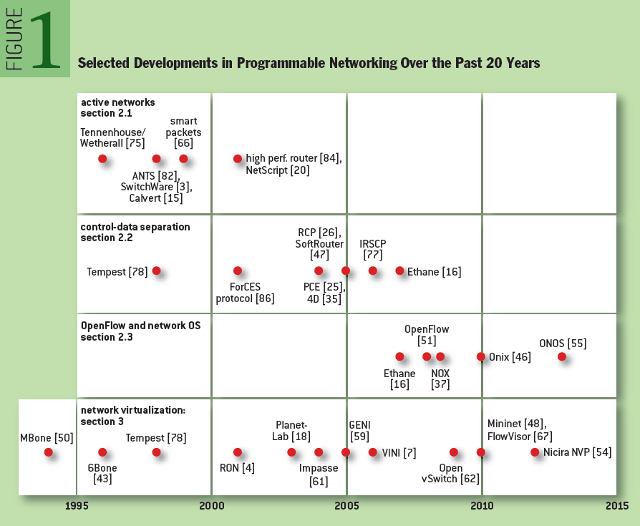
\includegraphics[width=15cm]{sdn-history}
    \caption{Desarrollos selectos en el campo de redes programables en los últimos 20 años. Tomado de \emph{The Road to SDN}\cite{rexford}.}
    \label{fig:tradicitional-architecture}
\end{figure*}


\section{Software Defined Networks}

El \textit{Open Network Foundation} -- la organización encargada de promover la implementación de redes SDN y estándares para las mismas - define SDN como la separación física del plano de control (\emph{control plane}) de la red del plano de datos o reenvío (\emph{forwarding plane}), en donde un plano de control controla varios dispositivos\cite{onf}. 

El objetivo de las redes SDN es brindar una interfaz abierta que pueda permitir el desarrollo de software para controlar la conectividad dentro de una red, el flujo y el tráfico.
La idea central es desacoplar el control de la red del de datos y que además sea programable. Al tener una separación entre la parte lógica y la física se busca abstraer los servicios y las aplicaciones los cuales pueden tratar la red como una entidad lógica o virtual. 


\subsection{Arquitectura}
Los dispositivos de red tradicionales, como un \emph{switch}, tiene 3 planos: el plano de administración, el plano de control y el plano de datos. El plano de administración permite la configuración del dispositivo y el de control, que controla el enrutamiento del tráfico. La tabla de ruteo la llena el plano de control (por un algoritmo de enrutamiento) que a su vez determina cómo el tráfico debería ser enrutado por el hardware. Finalmente, la capa de datos se encarga de este enrutamiento. Uno de los problemas con las redes tradicionales, el cual SDN está intentando cambiar, es que cada dispositivo en la red tiene su propio plano de administración, control y de datos. Si la red tiene 100 \emph{switches}, entonces se tienen 100 planos de administración, 100 de control y 100 de datos. Se tiene que administrar cada dispositivo por separado, cada uno ejecutando un algoritmo distribuido de enrutamiento como \emph{Open Shortest Path first}(OSPF) que tiene que determinar la mejor ruta de un punto de la red al otro y que, con suerte tendrá conocimiento completo de la red o al menos uno bueno de la misma. OSPF y otros algoritmos distribuidos de enrutamiento son complejos y no necesariamente elijen la mejor ruta porque no tienen una vista del tamaño total de la red. 

\begin{figure}[h]
    \centering
    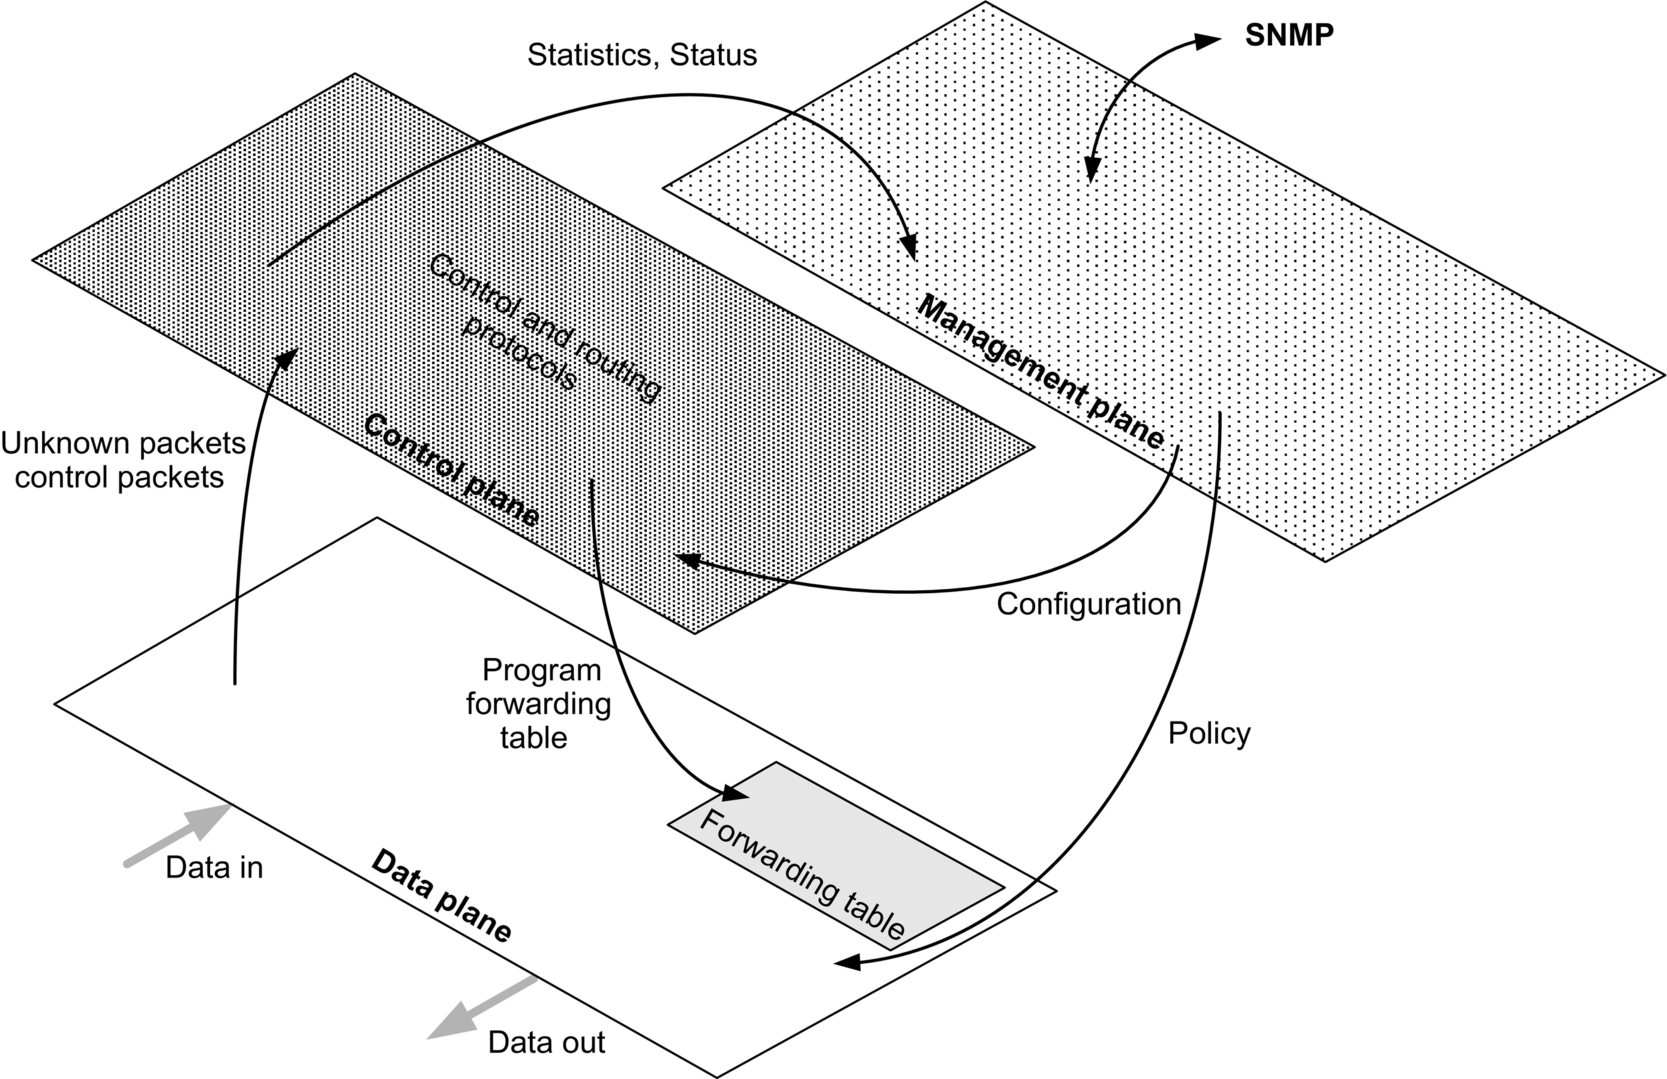
\includegraphics[width=8cm]{traditional-3-tier-device}
    \caption{Arquitectura de un dispositivo tradicional. Fuente: \emph{Software Defined Networks}\cite{goransson}.}
    \label{fig:tradicitional-architecture}
\end{figure}




Con SDN, la idea es remover el ``cerebro'' o la ``inteligencia'' del dispositivo de red y llevarlo a un dispositivo diferente como un \textbf{controlador:} un dispositivo que actúa como un punto de control estratégico -- probablemente compuesto de varios servidores físicos- que controla varios dispositivos de red tanto físicos como virtuales y que tiene mejor conocimiento de la red porque es un único ente controlando la totalidad de red o una porción de la misma. Protocolos como \textsc{OpenFlow} permiten al plano de control manipular el enrutamiento de tráfico a través de la red realizando mejores decisiones a la hora de calcular rutas y de gestionar de la red.

\begin{figure}[h]
    \centering
    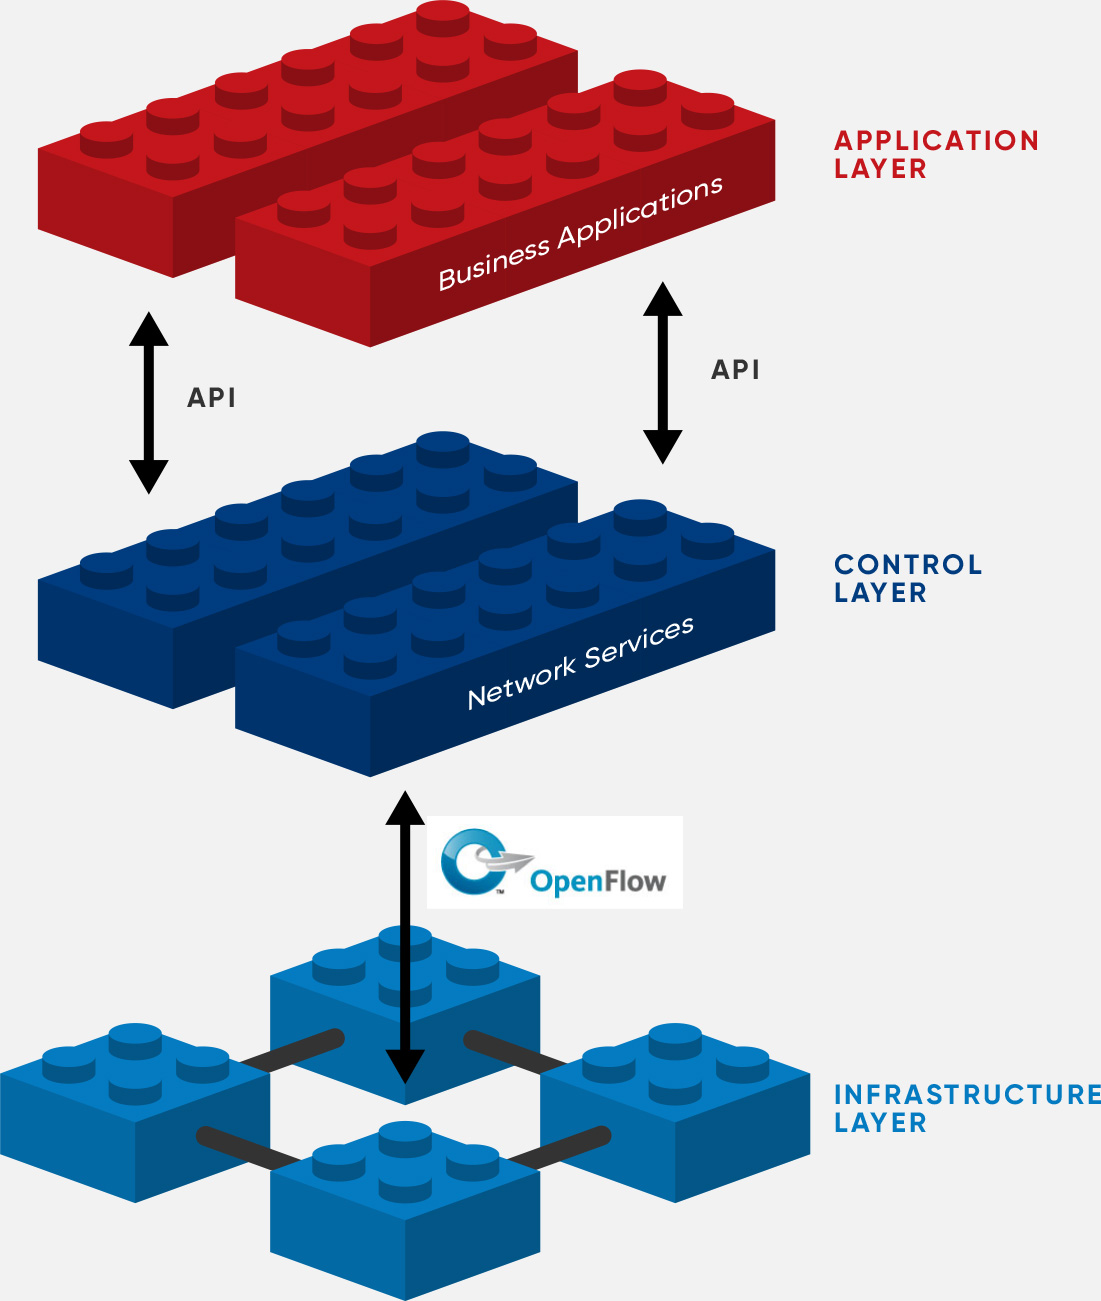
\includegraphics[width=8cm]{sdn-architecture-img}
    \caption{Arquitectura SDN. Fuente: \emph{Open Networking Foundation}}
    \label{fig:sdn-arquitectura}
\end{figure}


SDN define una arquitectura formada por tres capas distintas como se muestra en la figura \pageref{fig:sdn-arquitectura}:
\subsubsection*{Capa de infraestructura}
Se ubica el equipo físico de transferencia (\emph{routers, switches}, etc).

\subsubsection*{Capa de control}
Se encuentran los \textbf{controladores} SDN y aplicaciones escritas por programadores que interactúan con el controlador utilizando lo que se conoce como la interfaz \emph{Northboud}. Para interactuar con los dispositivos de la red, el controlador usa la interfase \emph{Softboud}. El controlador envía mensajes a los dispositivos usando varios protocolos -- Uno de ellos es \textsc{OpenFlow} - en la intefase \emph{Softbound}. A diferencia de un \emph{switch} o \emph{router} tradicional, en un ambiente SDN puro el cerebro del dispositivo de red es removido del mismo y se coloca en la capa de control en un dispositivo por separado.

%Es una entidad de software que controla la infraestructura de forma dinámica a través de solicitudes que vienen desde la capa de aplicación.
%Esta puede tomar soluciones informadas para configurar la capa de infraestructura con el fin de que esta sea óptima.
%La inteligencia de la red es manejada desde la capa de control logrando mantener una vista general de la red, teniendo como resultado un solo switch lógico que opera aplicaciones y políticas. 
%
%La capa de control puede proveer protocolos NetFlow, IPFIX, SNMP, entiende la topología de la red y provee enlaces entre dispositivos. 
%Se puede escalar para que exista más de un controlador para la red (Multiple control/data planes) donde ambos controladores se sincronizan para administrar la red, permitiendo la sincronización entre varios controladores, ``high availability'' y tolerancia a fallos.

\subsubsection*{Capa de aplicación}
Las aplicaciones en esta capa manipulan el flujo de tráfico a través de la red. SDN permite control sobre toda la red desde un solo punto lo cual simplifica el diseño y el mantenimiento de la red. También reduce el trabajo entre dispositivos de red pues solo necesitan recibir instrucciones de la capa de control en vez de entender y procesar distintos protocolos.

El trabajo de operadores de red también se ve reducido a solo mantener y configurar la capa de control, lo cual les da tiempo para aprovechar en la mejora de la red al implementar inteligencia para alterar el comportamiento de la misma de forma dinámica y responder a las necesidades de clientes. 

La arquitectura SDN soporta un conjunto de intefases de programación (API) para incluir servicios como ruteo, seguridad, control de acceso, manejo de rutas, distribución de cargas, entre otros. SDN promueve el uso de estas APIs que pueden ser de código abierto, dejando de lado el soporte de proveedores. Si por ejemplo se quisiera implementar un nuevo algoritmo de enrutamiento y ponerlo a disposición en los \emph{routers} de un cierto fabricante, este podría negarse a incluirlo. De la misma forma en la que el \emph{Apple Store} o \emph{Google Play} permiten a los programadores de aplicaciones a escribir sus propios programas al proveer interfaces de programación de alto nivel para tener acceso a los recursos de los teléfonos, una de las ideas de SDN es que un programador pueda escribir su propio programa y por medio de la interfaz \emph{Northbound} se pueda controlar el flujo del tráfico de la red. El controlador abstrae la complejidad detrás de la programación de la red y la interfaz abierta en los dispositivos de red permite que el programador controle, por medio del programa que escribió, el flujo del tráfico. Se podría utilizar un lenguaje de alto nivel como Python para programar los circuitos de los \emph{switches} sin tener que enviar mensajes de bajo nivel a dispositivos individuales en la red y cambiarle la configuración. La complejidad de la red se le oculta al programador: se puede escribir una aplicación de alto nivel que manipule el flujo de los datos a través de la red utilizando un protocolo como \textsc{OpenFlow} pero, la complejidad de \textsc{OpenFlow} y la complejidad de los dispositivos de la red están ocultos o abstraídos. De esta forma el programador solamente tiene que tener conocimiento una interfaz de alto nivel para escribir un programa manipule el envío de tráfico de un punto $a$ a un punto $b$.

\subsection{Características Fundamentales de SDN}

\subsubsection{Separación de planos}
La primer característica fundamenta de SDN es la separación de los planos de control y datos. Funcionalidades de reenvío (\emph{forwarding}) incluyendo las tablas lógicas y las tablas para escoger como lidiar con los paquetes entrantes, basados en características tales como una dirección MAC, dirección IP o una VLAN ID, reside en el plano de datos. Las acciones fundamentales realizadas por el plano de datos pueden ser descritas de acuerdo cómo manejan los paquetes que llegan. Se puede hacer \emph{forward, drop, consume} o \emph{replicate} un paquete entrante. También se puede transformar el paquete de alguna forma antes de tomar una acción posterior. 

La lógica y los algoritmos que son usado para programar el plano de datos reside en el control de datos. Muchos de estos protocolos y algoritmos requieren conocimiento global de la red. El plano de control determina cómo las tablas de reenvío (\emph{forwarding tables}) y la lógica en el plano de datos debería ser programada o configurada. En una red tradicional cada dispositivo tiene su propio plano de control, la tarea primaria de ese plano de control es ejecutar protocolos de ruteo y \emph{switching} de tal forma que todas las tablas de reenvío en los dispositivos en toda la red están sincronizadas.

\subsubsection{Dispositivos simples y control centralizado}
Los dispositivos son ahora controlados por un sistema centralizado ejecutando software de administración y control. En lugar de cientos o miles de líneas de complicado software de plano de control ejecutándose en el dispositivo y que le permite comportarse de forma autónoma, ese software es removido del dispositivo y puesto en un controlador centralizado. Este controlador basado en software puede entonces gestionar la red. El controlador provee instrucciones primitivas a los dispositivos simplificados cuando sea apropiado con el fin de permitirles hace decisiones más rápidas acerca de cómo manejas los paquetes entrantes.

\subsubsection{Automatización y virtualización de redes}
El controlador basado en software en SDN provee una interfaz abierta en el mismo para permitir el control automático de la red. En el contexto de Open SDN\footnote{Decir algo de esto - OpenSDN} los términos \emph{northbound} y \emph{southbound} se usan frecuentemente para distinguir si la interfaz es para las aplicaciones o para los dispositivos. Estos términos se derivan del hecho que en la mayoría de los diagramas las aplicaciones se muestra arriba (al norte) del controlador mientras que los dispositivos se muestra en la parte de abajo (al sur) del controlador. El controlador ofrece una \emph{northboud} API que permite que se pueda proporcionar algoritmos y protocolos que pueden hacer que la red trabaje eficientemente. La \emph{northbound} API del controlador pretende brindar una abstraccio4n de los dispositivos de red y la topología, de esta forma, las aplicaciones pueden ser desarrolladas para que trabajen sobre una amplia variedad equipos/fabricantes los cuales pueden diferir substancialmente en los detalles de su implementación.

Uno de los resultados de este nivel de abstracción es proveer la habilidad de virtualizar la red, desacoplar el servicio de la red de la red física subyacente. Esos servicios están aún presentes en los dispositivos \emph{host} de tal forma que esos \emph{hosts} no están concientes que los recursos de la red que están usando son virtuales o no los físico para los cuales fueron diseñados originalmente.

\subsubsection{Apertura}
Una característica de las redes SDN basadas en \textsc{OpenFlow} es que las interfases deberían de permanecer estándar, bien documentadas y no ser propietarias. Las APIs que son definidas deberían dar al software el suficiente control de varios planos de control. La premisa es que al mantener las interfases \emph{northbound} y \emph{southbound} abiertas en el controlador SDN se permitirá la investigación de nuevos e innovadores métodos para operar una red.

\subsection{Operativa de SDN}
A nivel conceptual, el comportamiento y operación de una red SDN es sencillo. En la figura \ref{fig:operation-sdn} se proporciona una representación gráfica de la operación de los componentes básicos de SDN: los dispositivos SDN, el controlador y las aplicaciones. La forma más fácil de entender la operación es mirándola de abajo hacia arriba, iniciando por los dispositivos. Los dispositivos SDN contienen funcionalidad de reenvio (\emph{forwarding}) para decidir qué hacer con cada paquete entrante. Los dispositivos también contienen los datos para tomar esas decisiones de reenvio. Los datos como tal son representados por los flujos definidos por el controlador, como se muestra en la parte superior izquierda de cada dispositivo.

\begin{figure}[h]
    \centering
    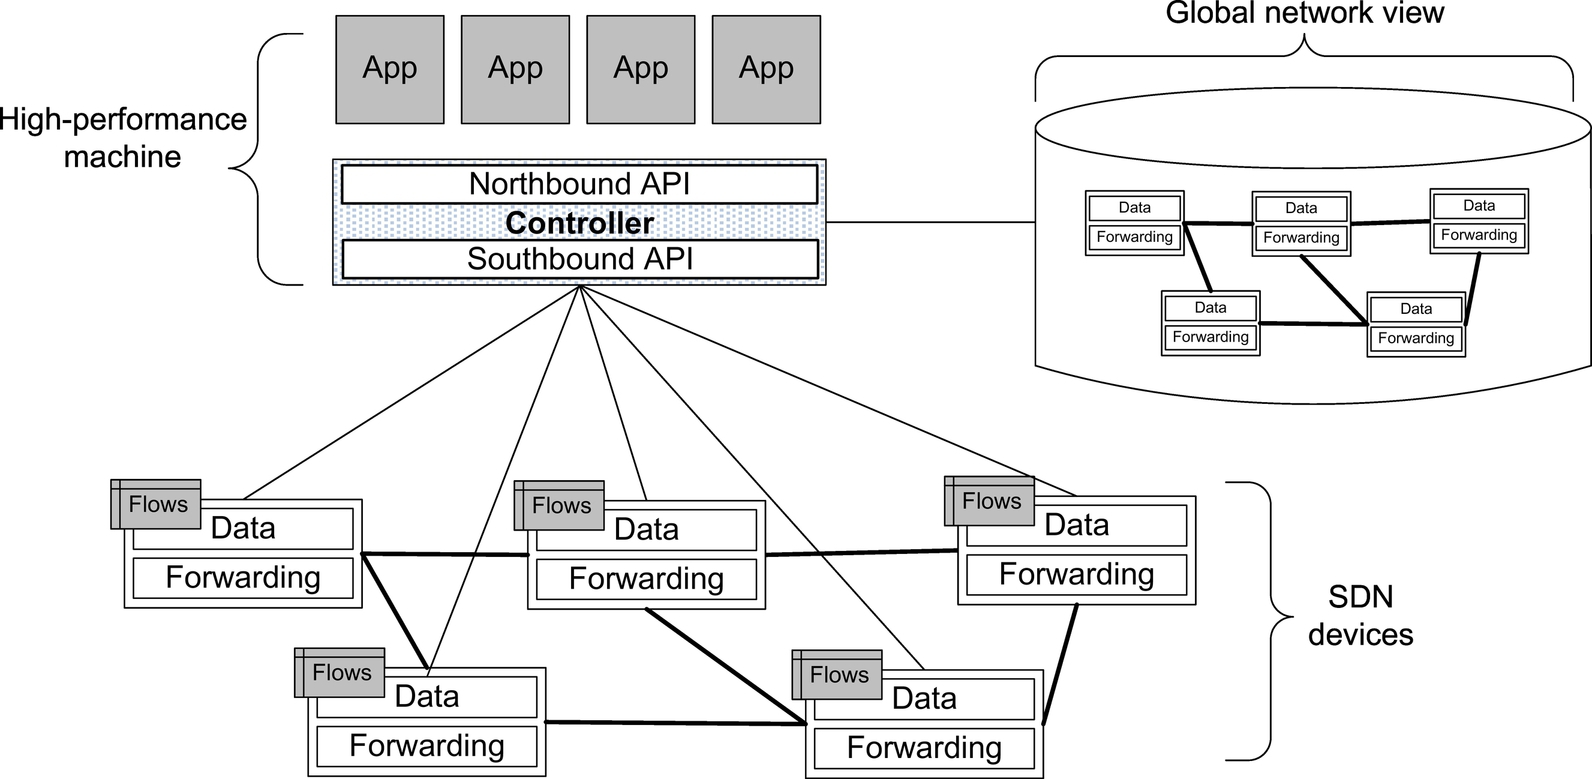
\includegraphics[width=9cm]{operation-sdn}
    \caption{Visión general de la operativa SDN. Fuente: \emph{Open Networking Foundation}}
    \label{fig:operation-sdn}
\end{figure}

Un flujo describe un conjunto de paquetes transferidos desde un punto final de la red (\emph{network endpoint}) hacia otro punto final de la red (o conjunto de puntos). Un conjunto de reglas describe las acciones que el dispositivo debería toma para todos los paquetes que le pertenecen a ese flujo. Un flujo \emph{flow} es unidireccional en que los paquetes que fluyen entre los mismos dos \emph{endpoints}, en la dirección opuesta podrían constituir cada uno un flujo separado. Los flujos se representan en un dispositivo como una entrada de flujo (\emph{flow entry}).

Una tabla de flujos reside en el dispositivo de red y consiste de una serie de entradas de flujo y las acciones a realizar cuando un paquete entrante coincide un flujo. Cuando el dispositivo SDN recibe un paquete, consulta su tabla de flujos en busca de una coincidencia. Estas tablas de flujos se han construido previamente cuando el controlador descargó las reglas de flujo apropiadas al dispositivo. Si el dispositivo SDN encuentra una coincidencia entonces realiza la acción configurada apropiada que usualmente implica reenviar un paquete. Si no encuentra una coincidencia, el dispositivo puede soltar (\emph{drop}) el paquete o pasarlo al controlador, dependiendo de la versión el protocolo y la configuration que tenga. La definición de un flujo es una expresión de programación relativamente simple de lo que lo que puede ser un cálculo de plano de control muy complejo realizado previamente por el controlador.

El controlador SDN es responsable de abstraer la red de los dispositivos SDN que controla y presentar una abstracción de estos recursos de red a las aplicaciones SDN ejecutándonse por encima de sí. El controlador le permite a las aplicaciones SDN a definir flujos en los dispositivos y ayuda a la aplicación a responder a paquetes que fueron reenviados al controlador por los dispositivos SDN. En la figura \ref{fig:operation-sdn} se puede ver en la parte derecha del controlador que se mantiene una vista de la totalidad de la red que controla. Esto permite calcular soluciones de reenvio óptimas de una forma determinística y predecible. Debido a que un controlador puede control un gran número de dispositivos, estos cálculos son normalmente realizados en un equipo de alto rendimiento el cual posee mejor CPU y memoria que los que vienen típicamente en los dispositivos de red.

Las aplicaciones SDN están construidas por encima del controlador. Estas aplicaciones no deberían de confundirse con la capa de aplicación definida en el modelo OSI de siete capas para redes de computadoras. Las aplicaciones SDN se interconectan con el controlador usando un conjunto de flujos proactivos (\emph{proactive}) en los dispositivos y para recibir paquetes que han sido enviados al controlador. Los flujos proactivos los establece la aplicación: típicamente la aplicación va a configurar estos flujos cuando la aplicación inicia. Los flujos van a persistir hasta que algún cambio en la configuracion se haga. Esta clase de flujo se conoce como flujo estático. Otro tipo de flujo proactivo es cuando el controlador decide modificar un flujo basado en la carga del tráfico que se está dando actualmente a través del dispositivo de red.

Además de los flujos definidos proactivamente por la aplicación, algunos flujos son definidos para responder a un paquete enviado al controlador. Al recibir los paquetes entrantes que han sido reenviados al controlador, la aplicación SDN dara instrucciones al controlador para darle a conocer cómo responder al paquete y, si es apropiado, establecerá nuevos flujos en el dispositivo con el fin de permitir que el dispositivo responda localmente la próxima vez que vea un paquete que le pertenezca a ese flujo. Tales flujos se llaman flujos reactivos. De esta forma, ahora es posible escribir aplicaciones de software que implementan envío, ruteo, superposición (\emph{overlay}), \emph{multipath}, funciones de control de acceso, entre otros.

\subsubsection{Dispositivos SDN}

\subsubsection{Controlador SDN}

\subsubsection{Aplicaciones SDN}


%\textbf{======================================}
%Control: se encuentran los controladores SDN y aplicaciones escritas por programadores que interactúan con el controlador utilizando lo que se conoce como la interfase \emph{Northboud}. Para interactuar con los dispositivos de la red, el controlador usa la interfase \emph{Softboud}. El controlador envía mensajes a los dispositivos usando varios protocolos -- Uno de ellos es \textsc{OpenFlow} - en la intefase \emph{Softbound}. A diferencia de un \emph{switch} o \emph{router} tradicional, en un ambiente SDN puro el cerebro del dispositivo de red es removido del mismo y se coloca en la capa de control en un dispositivo por separado.

 




%El dispositivo se puede acceder por medio de la terminal (\texttt{telnet}) y la interfaz de línea comandos que provee el fabricante para su configuración. Estas son funciones de administración: se cambia el comportamiento del dispositivo a través de su configuración. En el dispositivo también se puede habilitar un protocolo de enrutamiento. Los protocolos de enrutamiento actúan como protocolos del plano de control: cambian la forma en lo que paquetes son enrutados a través de la red. Estos protocolos no cambian la configuración del dispositivo, solamente cambian el comporamiento de enrutamiento, administran las tablas de ruteo las cuales determinan cómo los paquetes fluyen por el dispositivo.




\section{El Protocolo OpenFlow}
\textsc{OpenFlow} es el primer protocolo estándar que trabaja entre la capa de control. Permite el acceso directo y el manejo de los dispositivos físicos o virtuales. El protocolo especifica primitivas básicas que pueden ser usadas por aplicaciones externas para programar los dispositivos de  red. Por ejemplo, un programa que se cree para controlar la carga de red puede implementar OpenFlow para crear la comunicación entre los dispositivos de la red y el software, similar a las instrucciones de CPU que interactúan entre el sistema operativo y el hardware. 

El protocolo permite también definir como el tráfico de la red en base a parámetros como patrones de uso, aplicaciones y recursos de la nube. Provee un control granular que permite a la red responder a cambios en tiempo real a nivel de aplicación, usuario y sesión. 

Actualmente es el único protocolo de SDN estandarizado que permite la manipulación de la red.  

Parte de los beneficios de usar este protocolo está la centralización del control de ambientes de diferentes proveedores de dispositivos físicos/virtuales, reducir la complejidad del mantenimiento de la red mediante la automatización de procesos, innovación al permitir al programador crear aplicaciones según las necesidades del negocio, aumenta la seguridad de la red pues permite una configuración de alto nivel de políticas de seguridad, configuraciones dinámicas aplicables en pocas horas que reducen el \emph{``time-to-market''} del negocio, control granular de la red al aplicar políticas o configuraciones según diferentes niveles de distribución y carga.

\subsection{Otros protocolos e iniciativas}



% needed in second column of first page if using \IEEEpubid
%\IEEEpubidadjcol


% An example of a floating figure using the graphicx package.
% Note that \label must occur AFTER (or within) \caption.
% For figures, \caption should occur after the \includegraphics.
% Note that IEEEtran v1.7 and later has special internal code that
% is designed to preserve the operation of \label within \caption
% even when the captionsoff option is in effect. However, because
% of issues like this, it may be the safest practice to put all your
% \label just after \caption rather than within \caption{}.
%
% Reminder: the "draftcls" or "draftclsnofoot", not "draft", class
% option should be used if it is desired that the figures are to be
% displayed while in draft mode.
%
%\begin{figure}[!t]
%\centering
%\includegraphics[width=2.5in]{myfigure}
% where an .eps filename suffix will be assumed under latex, 
% and a .pdf suffix will be assumed for pdflatex; or what has been declared
% via \DeclareGraphicsExtensions.
%\caption{Simulation results for the network.}
%\label{fig_sim}
%\end{figure}

% Note that IEEE typically puts floats only at the top, even when this
% results in a large percentage of a column being occupied by floats.
% However, the Computer Society has been known to put floats at the bottom.


% An example of a double column floating figure using two subfigures.
% (The subfig.sty package must be loaded for this to work.)
% The subfigure \label commands are set within each subfloat command,
% and the \label for the overall figure must come after \caption.
% \hfil is used as a separator to get equal spacing.
% Watch out that the combined width of all the subfigures on a 
% line do not exceed the text width or a line break will occur.
%
%\begin{figure*}[!t]
%\centering
%\subfloat[Case I]{\includegraphics[width=2.5in]{box}%
%\label{fig_first_case}}
%\hfil
%\subfloat[Case II]{\includegraphics[width=2.5in]{box}%
%\label{fig_second_case}}
%\caption{Simulation results for the network.}
%\label{fig_sim}
%\end{figure*}
%
% Note that often IEEE papers with subfigures do not employ subfigure
% captions (using the optional argument to \subfloat[]), but instead will
% reference/describe all of them (a), (b), etc., within the main caption.
% Be aware that for subfig.sty to generate the (a), (b), etc., subfigure
% labels, the optional argument to \subfloat must be present. If a
% subcaption is not desired, just leave its contents blank,
% e.g., \subfloat[].


% An example of a floating table. Note that, for IEEE style tables, the
% \caption command should come BEFORE the table and, given that table
% captions serve much like titles, are usually capitalized except for words
% such as a, an, and, as, at, but, by, for, in, nor, of, on, or, the, to
% and up, which are usually not capitalized unless they are the first or
% last word of the caption. Table text will default to \footnotesize as
% IEEE normally uses this smaller font for tables.
% The \label must come after \caption as always.
%
%\begin{table}[!t]
%% increase table row spacing, adjust to taste
%\renewcommand{\arraystretch}{1.3}
% if using array.sty, it might be a good idea to tweak the value of
% \extrarowheight as needed to properly center the text within the cells
%\caption{An Example of a Table}
%\label{table_example}
%\centering
%% Some packages, such as MDW tools, offer better commands for making tables
%% than the plain LaTeX2e tabular which is used here.
%\begin{tabular}{|c||c|}
%\hline
%One & Two\\
%\hline
%Three & Four\\
%\hline
%\end{tabular}
%\end{table}


% Note that the IEEE does not put floats in the very first column
% - or typically anywhere on the first page for that matter. Also,
% in-text middle ("here") positioning is typically not used, but it
% is allowed and encouraged for Computer Society conferences (but
% not Computer Society journals). Most IEEE journals/conferences use
% top floats exclusively. 
% Note that, LaTeX2e, unlike IEEE journals/conferences, places
% footnotes above bottom floats. This can be corrected via the
% \fnbelowfloat command of the stfloats package.




\section{Conclusion}
The conclusion goes here.





% if have a single appendix:
%\appendix[Proof of the Zonklar Equations]
% or
%\appendix  % for no appendix heading
% do not use \section anymore after \appendix, only \section*
% is possibly needed

% use appendices with more than one appendix
% then use \section to start each appendix
% you must declare a \section before using any
% \subsection or using \label (\appendices by itself
% starts a section numbered zero.)
%


\appendices
\section{Proof of the First Zonklar Equation}
Appendix one text goes here.

% you can choose not to have a title for an appendix
% if you want by leaving the argument blank
\section{}
Appendix two text goes here.


% use section* for acknowledgment
\ifCLASSOPTIONcompsoc
  % The Computer Society usually uses the plural form
  \section*{Acknowledgments}
\else
  % regular IEEE prefers the singular form
  \section*{Acknowledgment}
\fi


The authors would like to thank...


% Can use something like this to put references on a page
% by themselves when using endfloat and the captionsoff option.
\ifCLASSOPTIONcaptionsoff
  \newpage
\fi



% trigger a \newpage just before the given reference
% number - used to balance the columns on the last page
% adjust value as needed - may need to be readjusted if
% the document is modified later
%\IEEEtriggeratref{8}
% The "triggered" command can be changed if desired:
%\IEEEtriggercmd{\enlargethispage{-5in}}

% references section

% can use a bibliography generated by BibTeX as a .bbl file
% BibTeX documentation can be easily obtained at:
% http://www.ctan.org/tex-archive/biblio/bibtex/contrib/doc/
% The IEEEtran BibTeX style support page is at:
% http://www.michaelshell.org/tex/ieeetran/bibtex/
%\bibliographystyle{IEEEtran}
% argument is your BibTeX string definitions and bibliography database(s)
%\bibliography{IEEEabrv,../bib/paper}
%
% <OR> manually copy in the resultant .bbl file
% set second argument of \begin to the number of references
% (used to reserve space for the reference number labels box)
\begin{thebibliography}{1}

\bibitem{IEEEhowto:kopka}
H.~Kopka and P.~W. Daly, \emph{A Guide to \LaTeX}, 3rd~ed.\hskip 1em plus
  0.5em minus 0.4em\relax Harlow, England: Addison-Wesley, 1999.

\bibitem{onf}
Open Networking Foundation. \url{https://www.opennetworking.org/sdn-definition/}

\bibitem{rexford}
N.~ Feamster, J.~Rexford, and E.~Zegura. 2013. \emph{The Road to SDN}.\hskip 1em plus
  0.5em minus 0.4em\relax Queue 11, 12. December 2013.
  
\bibitem{goransson}
P.~Goransson and C.~Black. \emph{Software Defined Networks: A Comprehensive Approach}.\hskip 1em plus 0.5em minus 0.4em\relax Elsevier Science. 2016.
  
\end{thebibliography}

% biography section
% 
% If you have an EPS/PDF photo (graphicx package needed) extra braces are
% needed around the contents of the optional argument to biography to prevent
% the LaTeX parser from getting confused when it sees the complicated
% \includegraphics command within an optional argument. (You could create
% your own custom macro containing the \includegraphics command to make things
% simpler here.)
%\begin{IEEEbiography}[{\includegraphics[width=1in,height=1.25in,clip,keepaspectratio]{mshell}}]{Michael Shell}
% or if you just want to reserve a space for a photo:

\begin{IEEEbiography}[{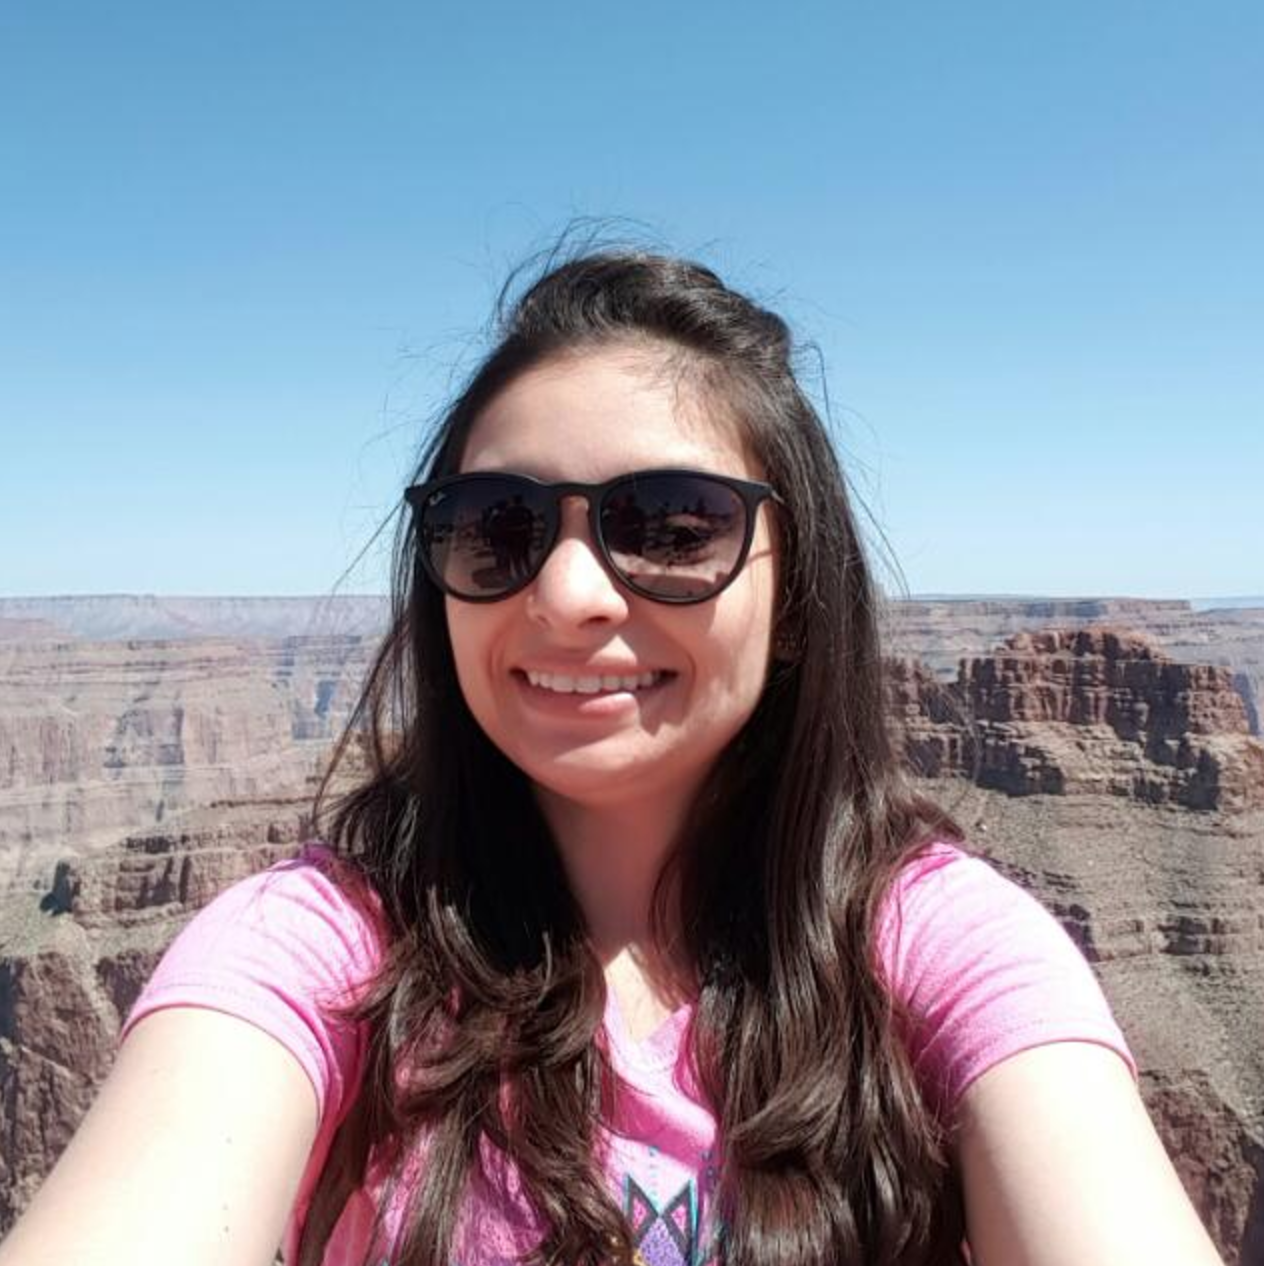
\includegraphics[width=1in,height=1.25in,clip,keepaspectratio]{priscilla-piedra}}]{Priscilla Piedra}
es Ingeniera de Computación del Instituto Tecnologíco de Costa Rica. Actualmente es estudiante del programa de maestría en Computación en la misma universidad. Sus principales intereses son: \emph{cloud computing} y automizatización. 
\end{IEEEbiography}

% if you will not have a photo at all:
\begin{IEEEbiography}[{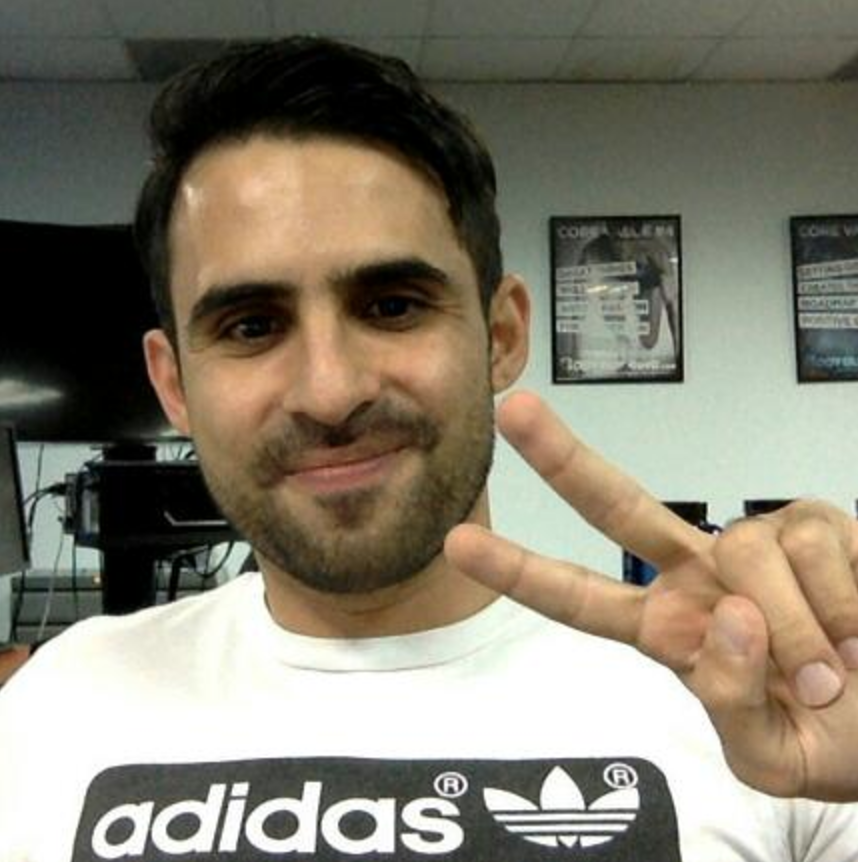
\includegraphics[width=1in,height=1.25in,clip,keepaspectratio]{martin-flores}}]{Martín Flores}
Biography text here.
\end{IEEEbiography}

% insert where needed to balance the two columns on the last page with
% biographies
%\newpage

%\begin{IEEEbiographynophoto}{Jane Doe}
%Biography text here.
%\end{IEEEbiographynophoto}

% You can push biographies down or up by placing
% a \vfill before or after them. The appropriate
% use of \vfill depends on what kind of text is
% on the last page and whether or not the columns
% are being equalized.

%\vfill

% Can be used to pull up biographies so that the bottom of the last one
% is flush with the other column.
%\enlargethispage{-5in}



% that's all folks
\end{document}


